\chapter{Introduction}
\label{ref:intro}

The standard model of particle physics (SM)
is the quantum field theory describing interactions of elementary particles,
namely quarks, leptons, and gauge bosons.
It has been successful in explaining many experimental results, such as parity
violation in weak interaction,
as well as predicting the existence of new particles, such as the Higgs boson.
%%%%
However,
there are experimental observations that cannot be explained by SM,
such as the existence of dark matter
which has no viable candidate in SM.
These observations demand new physics (NP).
One way to probe and constrain NP is through precision measurements
in which observables associated with certain processes are measured very
precisely and compared with predictions from SM.

One such process is semileptonic decay of the \B mesons:
$B \rightarrow D^{(*)} \ellm \neulb$,
where \ellm stands for a charged lepton which can be an electron $e^-$,
a muon \mun, or a tau \taum.
SM predicts lepton flavor universality (LFU),
that is, leptons participate in SM processes with the same strength
except for Higgs mechanism through which the leptons acquire different masses.
Therefore,
the ratios\footnote{
    Throughout the thesis, charge conjugation is assumed.
    Also, the convention $\hbar = c = 1$ is used unless specified explicitly.
} of branching fractions \RD and \RDst,
collectively referred as \RDX, defined as:
\begin{equation}
    \RDX \equiv \frac{\BFDTau}{\BFDMu}
\end{equation}
will not be 1 only because \taum and \mun have different masses,
which serves as a probe to LFU.
Note that it is more advantageous to measure the ratios instead of absolute
branching fractions because the latter depends on additional SM parameters,
for example $V_{cb}$,
which add another source of uncertainty;
whereas the former (\RDX) have many parameters, both theoretical and
experimental, cancelled for they are shared between the nominator and
denominator, making the measurement more precise.

Since 2012, tensions have been reported between measured \RDX and SM
predictions.
Currently, the world average tensions stand at about $3 \sigma$,
as shown in \cref{fig:hflav}.
The LHCb collaboration reported its latest measurement on \RDX based on LHCb run
1 (2011--2012) data very recently
(labelled as \emph{LHCb22} in the same figure).
The first part of the thesis is about a preliminary update of the LHCb run 1
measurement with LHCb 2016 data.

The LHCb detector is undergoing an upgrade as of now\footnote{
    ``Now'' is defined as Nov 2022.
} which greatly increases
the readout bandwidth of the detector and removes the hardware trigger along
with the limitations that come with it.
We the University of Maryland group are actively participating in the upgrade
of the Upstream Tracker (UT), a part of the tracking system.
The second part of the thesis will provide an overview of the LHCb upgrade, with
a focus on the UT readout system.

\begin{figure}[htb]
    \centering
    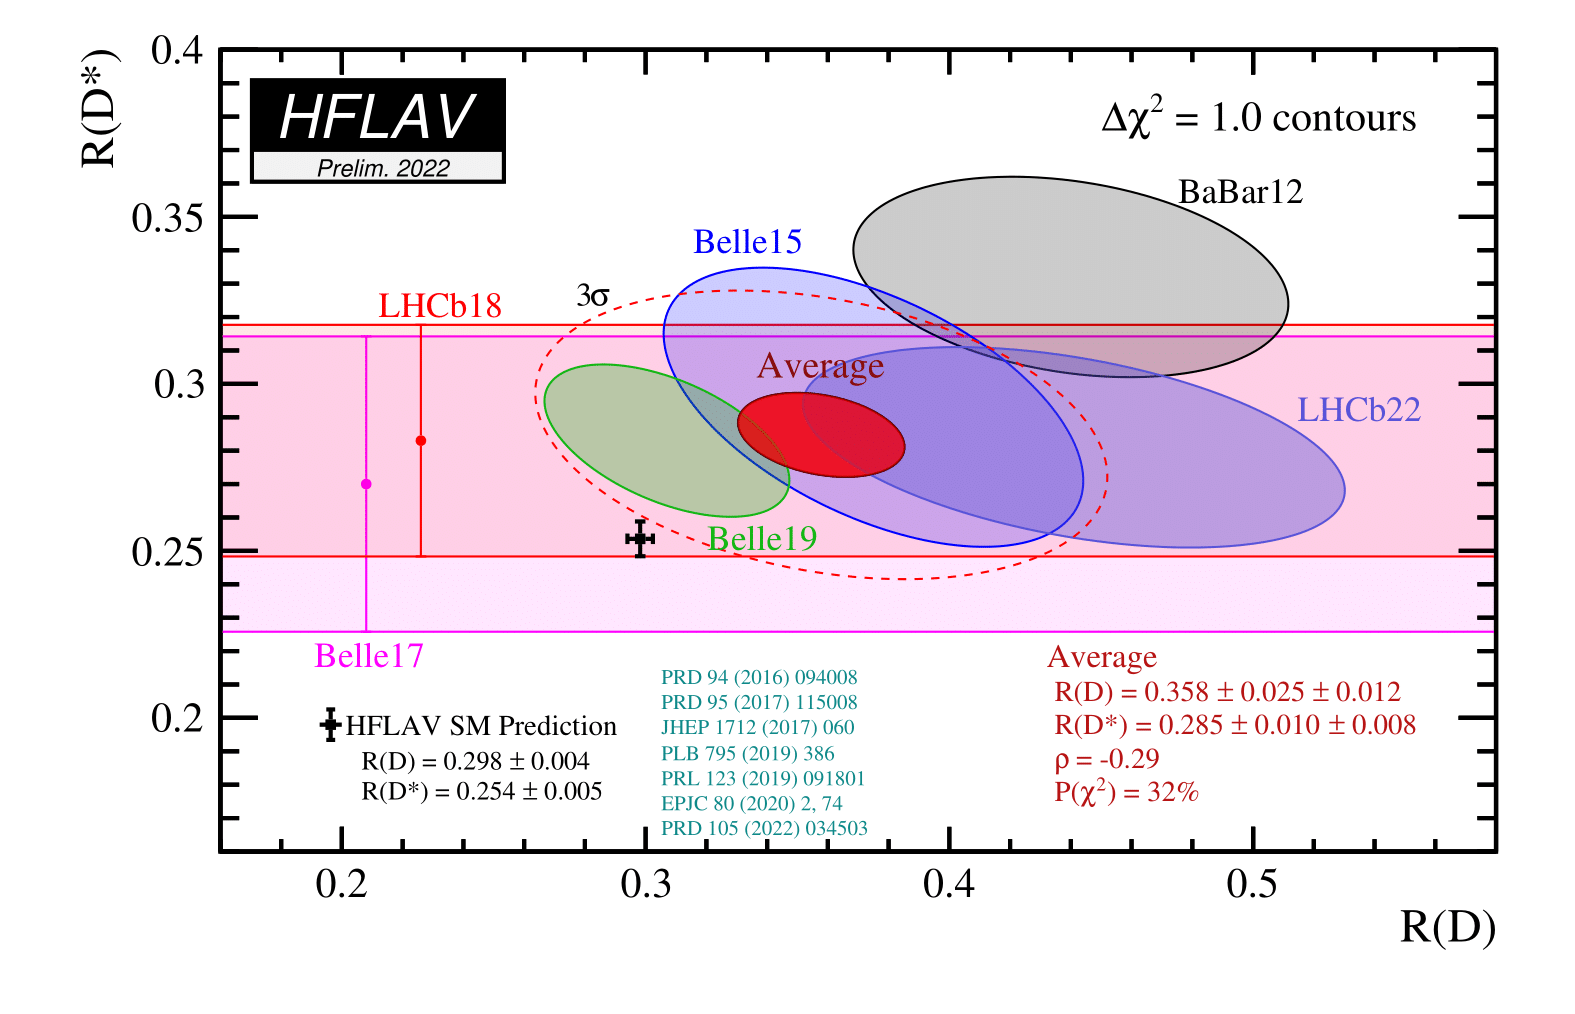
\includegraphics[width=0.6\textwidth]{./figs-intro/hflav_2022_preliminary.png}
    \caption{
        World average of \RD and \RDst, as of Nov 2022.
        Preliminary result from LHCb run 1 measurement is displayed as
        \emph{LHCb 22}.
    }
    \label{fig:hflav}
\end{figure}
